% THIS IS SIGPROC-SP.TEX VERSION 3.1
% WORKS WITH V3.2SP OF ACM_PROC_ARTICLE-SP.CLS
% APRIL 2009
%
% It is an example file showing how to use the 'acm_proc_article-sp.cls' V3.2SP
% LaTeX2e document class file for Conference Proceedings submissions.
% ----------------------------------------------------------------------------------------------------------------
% This .tex file (and associated .cls V3.2SP) *DOES NOT* produce:
%       1) The Permission Statement
%       2) The Conference (location) Info information
%       3) The Copyright Line with ACM data
%       4) Page numbering
% ---------------------------------------------------------------------------------------------------------------
% It is an example which *does* use the .bib file (from which the .bbl file
% is produced).
% REMEMBER HOWEVER: After having produced the .bbl file,
% and prior to final submission,
% you need to 'insert'  your .bbl file into your source .tex file so as to provide
% ONE 'self-contained' source file.
%
% Questions regarding SIGS should be sent to
% Adrienne Griscti ---> griscti@acm.org
%
% Questions/suggestions regarding the guidelines, .tex and .cls files, etc. to
% Gerald Murray ---> murray@hq.acm.org
%
% For tracking purposes this is V3.1SP APRIL 2009

\documentclass{acm_proc_article-sp}
\usepackage{balance}
\usepackage{graphicx}

\begin{document}

\title{Zero-Footprint Data Center Network Monitoring How to Monitor Your Data Center Networks for Free}
\subtitle{[Extended Abstract]}

\numberofauthors{3} 
\author{
\alignauthor
Author One\titlenote{sample titlenote}\\
       \affaddr{Institute One}\\
       \affaddr{Address One}\\
       \email{author.one@emails.com}
\alignauthor
Author Two\\
       \affaddr{Institute Two}\\
       \affaddr{Address Two}\\
       \email{author.two@emails.com}
%\and % go to new row
\alignauthor
Author Three\\
       \affaddr{Institute Three}\\
       \affaddr{Address Three}\\
       \email{author.three@emails.com}
%\alignauthor
%Author Four\\
%       \affaddr{Institute Four}\\
%       \affaddr{Address Four}\\
%       \email{author.four@emails.com}
}


\date{20 April 2013}

\maketitle

\balance

\begin{abstract}
(We should give a cool name to refer this system)

This paper present a network monitoring architecture which take advantages of Software Defined Network and traditional monitor methods. Our architecture support the a number of features: 1)monitoring both large and small flows with low cost, 2)adjust the work condition automatically according to the flow status, 3)accept instructions from users and other applications to control the flow, 4)combined with traditional detection methods.

optional: 1)support long-term flow analysis...
TODO: make features clearly
\end{abstract}

% A category with the (minimum) three required fields
%\category{H.4}{Information Systems Applications}{Miscellaneous}
%A category including the fourth, optional field follows...
%\category{D.2.8}{Software Engineering}{Metrics}[complexity measures, performance measures]

\terms{Application}

\keywords{network monitor, openflow} % NOT required for Proceedings


\section{Introduction}
%In modern datacenters, collecting the network flow statistics information and DPI information is important for attack detection and resource allocation. By monitoring the network flows, we could know whether there's irregular flows, which part is the most active and when to upgrade the whole system. If the bandwidth demands of servers and applications are changing dynamically, it is too difficult to give reasonable predictions and only real-time monitoring is feasible.\\
%However, the procedure of monitor all the network flows usually cost too much and we have to make a compromision between efficiency and accuracy.\\ 
%(TBA) More details\\
%(TBA)Our main contribution.\\

Network monitoring system is considered an indispensable part of the network infrastructure. By probing the instant network states and status, various network monitoring tasks provide useful information for network debugging, health check, intrusion detection, and application identification. More important, it is the most critical link for a closed loop control over the networks. For example, security policy enforcement such as intrusion prevention, traffic engineering for optimized network utilization, and access control for quality of services all rely on the information acquired from a network monitoring system. The advent of Software Defined Networking (SDN) offers fresh opportunities to such a closed loop system, in which a logical central controller provides a unique vantage point to oversee the entire network, analyze the data collected, and apply fine-grained controls on routing and policies based on the network states.\\
Data center is central to modern ICT (Information and Communication Technology) clouds. Within it, network acts as the artery of the infrastructure to provide connectivity for computing and storage nodes. The network’s health and performance is therefore critical to the service offered by the data center. However, data centers also face some challenges to support effective and efficient network monitoring.\\
First, data center is constantly under the pressure of power and cost. Meanwhile, the monitoring tasks are of great quantity and diverse a lot. Specialized and heterogeneous boxes dedicated for network monitoring significantly increase the data center cost and power budget.
Second, data center can support multiple tenants or present complex work load patterns which makes the network data hard to analyze and the network behavior hard to predict. An agile network monitoring system needs to be able to collect and analyze the network traffic, and react in real time. The monitoring must also not negatively interfere with the normal network operation.\\
Third, data center is evolving into a “software-defined everything” age. The tools involved in network monitoring need to be unified and streamlined with other tools across
networking and computing. In order to lower and the operation cost and avoid incurring sheer learning curve, it is ideal to be able to integrate popular and open-source based software tools into the monitoring system with ease.\\
Last but not the least, data centers grow at a very fast pace. The monitoring system needs to be stable and scalable, and have a clear growth path as well. It would be counterproductive and even detrimental to the business if the monitoring subsystem upgrades always require a system-wide overhaul.\\
Traditionally, there are several different ways to handle the network monitoring tasks within data centers.\\
\begin{itemize}
\item Using standard or proprietary protocols such as SNMP\cite{SNMP}, NetFlow\cite{NetFlow}, and sFlow\cite{sflow}. Most of the existing network switches have built-in support for some popular network monitoring and management protocols. They are useful but not general enough to meet all monitoring requirements. For example, they are not accurate enough for many measurement tasks due to the randomly sampling nature. They are also unreliable for most of the security-related monitoring tasks since most of the packets are basically invisible to the monitoring system.
\item Tapping network and using specialized hardware-based fabric to deliver the traffic to different tools for analyzing (e.g. packet broker\cite{packetbroker}, BigTap\cite{bigtap}, Gigamon\cite{gigamon}). The so-called NPM (Network Performance Monitoring) and NPB (Network Packet Broker) systems are purposely built and can offer very high performance. The monitoring subsystem often operates in a separate shadow network but it does need the network switches to provide dedicated TAP (Test Access Point) or SPAN (Switch Port Analyzer) ports. What can be seen is limited by the switch capability. The extra hardware also incurs high capital and operating cost.
\item Using specialized hardware boxes either sits in line (e.g. hardware firewall\cite{hardware} and ADC appliances\cite{adc1,adc2}) or replacing the commodity off-the-shelf switches with more powerful and sophisticated ones with enhanced processing power for in-device monitoring (e.g. Servone\cite{servone} and Pluribus\cite{pluribus}). While no shadow network is needed, this one asks for new hardware and is fundamentally a proprietary network monitoring solution.
\end{itemize}
Instead of following old suit, our approach is drastically different. We provides a general DCN monitoring framework which overcomes the drawbacks of the previous approaches. The resulting monitoring system is non-intrusive, elastic, and scalable. It requires no extra investment on hardware and allows both open source and proprietary software to be seamlessly integrated together. Our approach is motivated by several recent trends in networking domain.\\
\begin{itemize}
\item SDN and OpenFlow\cite{openflow}: SDN advocates open programmability. It allows new network applications to be written in software and deployed into the forwarding plane devices through an open interface. This is unthinkable before for the vertically integrated network devices. It’s believed that Data Center will be the first place to apply SDN technologies. As a de factor south bound interface standard, OpenFlow can configure and control the switches’ behavior and pull their status and statistics at arbitrary flow level. The multi-table feature provides us a convenient way to embed monitoringrelated functions and features without interfering with the normal packet forwarding functions.
\item OCP and white-box switches\cite{ocp}: Open Compute Project aims to standardize the data center hardware components. Specifically, the OCP networking project promotes the white-box switches with open operating system and network stacks. These switches are widely available, low cost, and programmable. It gives the network operators great flexibility to customize the switch functions. When an OpenFlow agent is installed, these switches are easily converted into SDN switches.
\item NFV\cite{nfv}: First initiated by telecommunication service providers, Network Function Virtualization tries to realize various network functions using commodity servers and IT vitualization technologies to replace proprietary network devices. The significant performance boost of servers and their cost advantage make this idea plausible. By doing so, network operators can avoid vendor lock-in, roll out new services more quickly, and scale services smoothly. The proposal has created considerable traction in industry. The specialized middle-boxes such as firewall and IPS are among the first group of network gears which are losing ground.
\end{itemize}
To summary, our approach uses OpenFlow to control whitebox switches and realizes NFV-based network monitoring functions by orchestrating the white-box switches and commodity servers.
In a bigger picture, our system can be a monitoring-as-a-service framework in a software-defined data center\cite{software-} setup which is responsible for providing various services such as policy enforcement, performance tuning, intrusion detection, fault diagnosis, and other data mining tasks.\\
(Does it has anything to do with OpenStack?)\\
Section 2 details the architecture of our system.\\

\section{Architecture}
As we have emphasized, our data center monitoring system incurs no extra hardware investment and totally relies on the existing infrastructure, such as the surplus computing and networking resources which are in idle otherwise. [We need to gather some data to show that typical data center has enough redundant or idle resources to allow such a system] Therefore, effectively our data center monitoring system has zero footprint. Figure 1 illustrates the high level system overview.\\
\begin{figure}[htbp]
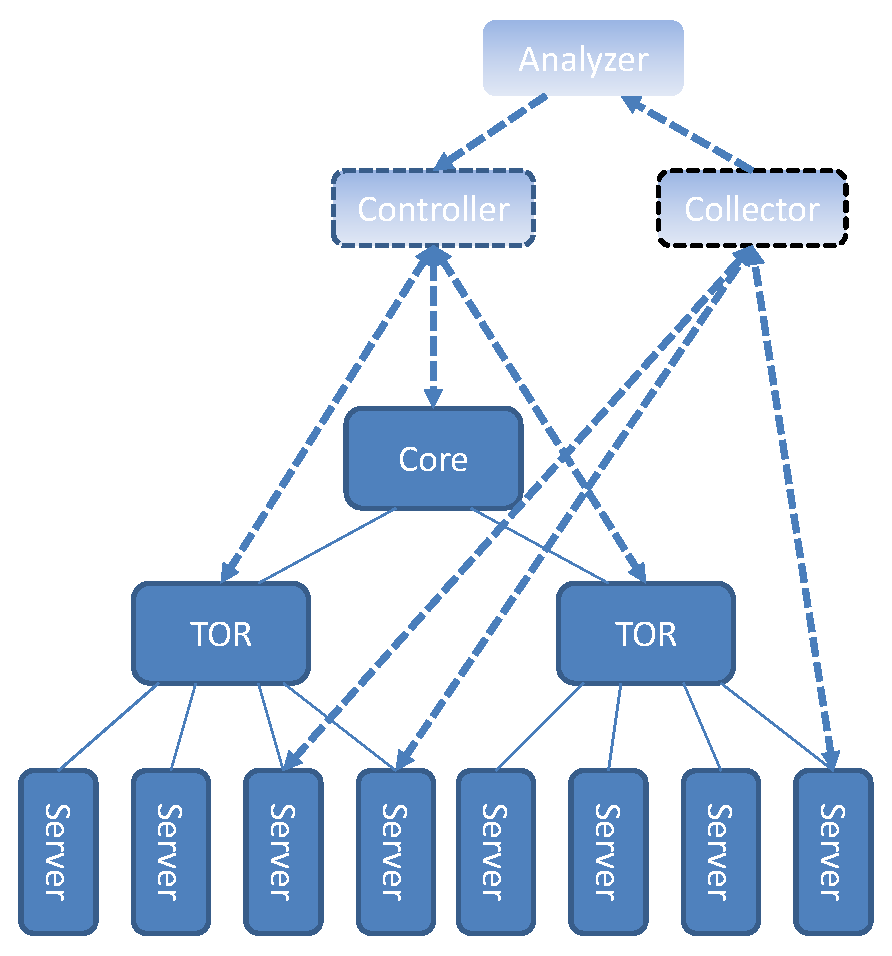
\includegraphics[width=3in]{image/arch}
\caption{Latency-L2}\label{fig:latency-l2}
\end{figure}
We assume the data center network is built with SDNenabled white-box switches. The SDN controller uses OpenFlow protocol to control the switches to conduct some monitoring related work in addition to normal packet forwarding. The system can dynamically designate some unused servers (or virtual machines in case a virtualized environment presents) as monitoring nodes. The TOR switch ports connecting to these servers are configured as mirror ports which can forward the selected traffic to the monitoring node for further investigation. The traffic filtering criteria for mirror ports are generated by the analyzer and deployed by the SDN controller. The monitoring nodes form a distributed system. Software running on the monitoring nodes performs different functions and returns results to the collector. The collector is responsible for configuring the functions on the monitoring nodes, and collecting and aggregating the results from the monitoring nodes. The aggregated results are then passed to the analyzer to consume. Based on the analysis results, different actions can be taken. For example, alerts can be raised, new rules can be generated, or new functions can be enabled. If new rules are generated, they are passed to the SDN controller through the controller’s north bound API. The controller can then reconfigure the switches to modify their behavior. We can see the components form a closed loop system. Note that the dashed boxes in Figure 1 are not specialized devices. They are also implemented in normal data center servers in racks. Each box can represent a single server or a server cluster, depending on the scale of the data center network and the monitoring system. Multiple boxes can also collocate in a single server.\\
\subsection{Switch configuration}
Each switch is configured as an OpenFlow switch. It should support OpenFlow 1.2 or newer versions in order to enable multi-table capability. In front of the normal forwarding pipeline, we insert one or more new flow tables dedicated for the monitoring subsystem. In addition to counting the matching packets, each flow entry can be configured to execute a few actions on matching packets including forwarding them to some mirror port or dropping them in place. Unless the packets are configured to be dropped, they will still be submitted to the normal forwarding pipeline. We will show that this simple mechanism allows a wide spectrum of monitoring applications to be efficiently conducted.\\
\subsection{Server configuration}
\subsection{Traffic collector and analyzer}
\subsection{Controller and Query language}

\section{Prototype and Test Bed}
\section{Use Cases}
\section{Experiments and Evaluation}


\section{Related Work}
(TBA)Related Work\\
Sample Citation:\\
openflow: \cite{openflow}\\
B4: \cite{google-b4}\\
csamp: \cite{csamp}\\
SIGCOMM14 switch mirroring Minlan Yu’s group
Diagnosis as a Service\cite{diagnosis}
The structure of the rest of this paper.

\section{Our Method}
(TBA)Brief summary of related work. Discuss the advantages and disadvantages of Sample, Mirror and so on.\\
(TBA, motivation)Now we consider the cost when we try to get the network flow information. If we use openflow table to monitor an point-to-point flow, the cost is one flow entry. If we mirror a flow to a server, the cost is the bandwidth. In our system, we use openflow entry to monitor large flow, and mirror small flows to the server.\\
The rest of the sections is arranged as follows. The system architecture part described the hardware architecture and flow table design, and why we build our system like this. The flow bandwidth monitor describes the algorithm and feedback control on filtering large flows and monitor small flows. The ddos attack detection describe how to monitor long-term ddos attack as well as short-term attack. The deep packetage information detection describe how we detect the package content by using other tools. And the operation for uses command part describe how can we follow users' instructions.\\

\subsection{System Architecture}
Hardware Structure

(image)\\
             user --> controller\\
             controller <--> switch\\
             switch ---> servers\\
             switch --> mirror server\\
             switch --> snort node(third-part tools)\\
             mirror server --> controller\\
             snort node --> controller\\
             (add port information, and link to controller is inband)\\


Briefly introduce the structure of different part and their relationships.\\
Briefly intrudoce the detailed structure of the controller.\\
Flow table Struction:\\
(image)\\
            flow table 1:\\
            ~~~~ for high level monitor (user different priority)\\
            flow table 0:\\
            ~~~~ for determinate flow monitor while can make routing decision by oneself (high priority)\\
            ~~~~ fow learning switch(low priority), inlucding the lowest priority packet-in\\

(TBA)Explain why use the high level part to monitor and routing, but not add another table. (Due to the hardware implentation of multi-table on Pica8...--Can we write like this?--)\\
(TBA)Explain why use table one for high level monitor. (It can't make routing decisions by one self. eg. all flow come from a given IP.)\\

\subsection{Flow Bandwidth Monitoring}
Bandwidth Detection:\\
Use flow entris to filter elephant flow.\\
Use feedback to adjust monitoring entries. If the mirror bandwidth extend the port bandwidth, times the factor for feedback result\\
\\
Flow Entry Replacement Algorithm\\
All use generated flow matrix to test. Easy to reappear.\\
Random vs Greedy vs Damping using long-term history and dft\\
compare target: mirror bandwidth,  monitor precision, entry change time and so on.\\
Use dft to detect whether the flow is mutable or stable. Combine it with the average flow size to determine whether to add the corresponding monitor entry.\\
Store long-term information also help to ddos detection.\\

\subsection{DDos attack detection}
Store all the flow statistics information of a period time.\\
For each src node and dst node, use the relavent flows to determine whether it is a potential attacker or a target.

\subsection{Deep Package Information Detection}
The shortage of our SDN monitor is we can't look up into the packets on the switch. Even we can look into the information in a packet when packet-in event happens, we can't affort the cost of packet-in. A general controller could only deal with 1k-10k packet-in request, which we will test later.\\
snort

\subsection{Operation for User Command}
Monitor Flows, Block Ports\\
Change work status.\\


\section{Evaluation}

\subsection{Environment Setup}
Hardware parameters introduction. Pica8-3295 and server models\\
Real System connection struction.\\

\begin{figure}[htbp]
\includegraphics[width=3in]{image/latency}
\caption{Latency-L2}\label{fig:latency-l2}
\end{figure}
\begin{figure}[htbp]
\includegraphics[width=3in]{image/bandwidth}
\caption{Bandwidth-L2}\label{fig:Bandwidth-l2}
\end{figure}

(Test is based on the features our method support, and including performance test.)

\subsection{Basic Environment Test}
Test on Switch and Controller:\\
Basic Test.\\
Use cbench or other tools. Test on standard learning switch between our switch.\\
(optional)Test the basic parameters of our system.

\subsection{Compared with L2}
Compare the Bandwidth and Latency under L2 and Openflow:\\
use scripts (got help from liyiran)\\
Test bandwidth between servers under L2 model and Openflow model. If these's little difference, change it to the test between L2 and openflow with our controller\\
(image)\\
Test bandwidth between servers under Openflow model with insert/delete monitor flows on different frequency.\\
(image)\\

Test the Bandwidth and Latency influence of inserting and deleting monitor flows.\\
Also test whether it lead to packet-loss when insert and delete flow entries.\\

\subsection{Precision}
Bandwidth(Elephant FLow):\\
Compared with sFlow.\\
Use generated flows, Compare the precision.\\
When bandwidth is not full, when mirror port is full.\\
absolute precision, precision compared with sflow.

DDoss:\\
Compared with?
absolute precision
long-term feature
react time

\subsection{Reaction Time}
The attack start time and detected time
DPI
user's command

\subsection{Cost, Cost includes flow entry, mirror bandwidth}
Use generated flows\\
Use real cluster flows(eg. Spark). Depends on the flow characteristc.


\section{Conclusion}
Conclusion\\


\bibliographystyle{abbrv}
\bibliography{sample}

\end{document}
